\def \secname {Fourier Transform}

\section[\secname]{\hyperlink{toc}{\secname}}



(following Numerical Methods, Press et al.)

\subsection{Quick Review}

\begin{itemize}
    \item Transform pairs: $h(t) \Longleftrightarrow H(f)$

    \[ h(at) \Longleftrightarrow \frac{a}{|a|} H(\frac{f}{|H|}\]

    \item Convolution

    \[ g*h \equiv \int_{-\infty}^{\infty} g(\tau) h(t-\tau)d\tau\]

    \[ g*h \Longleftrightarrow G(f)H(f) \quad \text{Convolution Theorem}\]

    \item Total Power 

    \[ \int_{-\infty}^{\infty} |h(t)|^2dt = \int_{-\infty}^{\infty} |H(f)|^2 df\]

    Parseval's Theorem

\end{itemize}

\subsection{FT of Discretely Sampled Data}

\subsubsection{Sampling Theorem and Aliasing}

\begin{itemize}
    \item Assume $h(t)$ sampled uniformly in time

    \[ h_n = h(\Delta n), \quad n=\ldots,-1,0,1,\ldots\]

    \item Sampling Rate: $\frac{1}{\Delta}$

    \item Nyquist Critical Frequency: $f_c = \frac{1}{2\Delta}$

    \begin{center}
        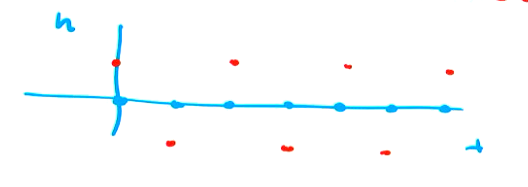
\includegraphics[width = 0.5 \linewidth]{Images/nyquist_aliasing.png}
    \end{center}

    \item Sampling Theorem: If continuous function h(t), samples at interval $\Delta$, its bandwidth limited to frequencies smaller than $f_c$ ($H(f) = 0$ for all $|f| \ge f_c$) then function is completely determined by its samples $h_n$

    \[ h(t) = \Delta \sum_{n=-\infty}^{+\infty} h_n \frac{\sin(2\pi f_c(t-n\Delta)}{\pi(t-n\Delta)}\]

    \item What happens if function is not bandwidth limited?

    \item All power spectral density outside nyquist range $-f_c < f < f_c$ is moved into that range $\Rightarrow$ \textbf{Alisasing}.

    \item Two waves exp($2\pi f,t$) and exp($2\pi f_c t$) yield same samples if and only if f, and $f_c$ by multiple of $\frac{1}{\Delta} \rightarrow$ width in frequency of range ($-f_c,f_c$)
\end{itemize}

\subsubsection{Discrete Fourier Transform}

\begin{itemize}
    \item Now what to estimate Fourier transform if a function from finite number of sample points.
    \item Suppose we have

    \[ h_k \equiv h(t_k), \qquad t_k = k\Delta, \quad k=0,1,\ldots, N-1\]

    Where $Delta$ is the spacing and $N$ is the number of samples.

    \item Will assume that N is even

    \item Seek estimates at discrete values

    \[ f_n = \frac{n}{N\Delta}, \qquad n = \frac{-N}{2}, \ldots , \frac{N}{2}\]

    \item Extreme values $\rightarrow$ lower and upper limits of the Nyquist critical frequency range

    \item Estimates for $n=-N/2,$ $N/2$ are equal $\Rightarrow$ there are a total of N independent $H_n$

    \[ H(f) = \int_{-\infty}^{\infty} h(t) e^{2\pi i f t} dt\]

    \item Approximate using discrete sum

    \begin{align}
        H(f_n) &= \int_{-\infty}^{\infty} h(t) e^{2 \pi i f_n t} \approx \sum_{k=0}^{N-1} h_k e^{2\pi i f_n t_n} \Delta \\
        &= \Delta \sum_{k=0}^{N-1} h_k e^{2\pi i k_n/N} 
    \end{align}

    \item Defines discrete Fourier Transform

    \begin{equation}
        H_n = \sum_{k=0}^{N-1} h_k e^{2\pi i k_n/N} 
    \end{equation}

    \item Have 

    \[ H(f_n) \approx \Delta H_n\]

    \item n value from -N/2 to N/2

    \item equation above is periodic in n with period N

    \[ \Rightarrow H_{-n} = H_{N-n}, \qquad n=1,2,\ldots\]

    \item Useful convention, let n take on values 0,1,2,..., N-1

    \begin{itemize}
        \item Zero frequency: n=0
        \item Positive frequency: n=1,2,...,N/2-1
        \item Negative frequency: n=N/2+1,N/2+2,...,N-1

        For Total of N samples 
        
    \end{itemize}

    \item Discrete inverse Fourier transform

    \[ h_k = \frac{1}{N} \sum_{n=0}^{N-1} H_n e^{-2 \pi i k_n/N}\]

    \item Discrete version of Parseval's Theorem

    \[ \sum_{k=0}^{N-1} |h_n|^2 =  \frac{1}{N} \sum_{n=0}^{N-1} |H_n|^2\]
\end{itemize}

\subsubsection{Fast Fourier Transform}

\begin{itemize}
    \item How much computation does it take to evaluate equation (73) above?

    \item Define complex number

    \[ w = e^{2\pi i/N}\]

    \item (73) can be written as

    \[ H_n = \sum_{k=0}^{N-1} w^{nk} h_k \]

    (exponent gives: nk-th power of w)
    
    \item In vector-matrix form

    \begin{equation}
        \mathbf{H} = \mathbf{A} \mathbf{h}
    \end{equation}

    \[ A_{ij} = w^{ij}\]

    \item (74) take $N^2$ multiplications and somewhat fewer operations to compute all $w^{ij}$

    \item Can actually evaluate FT in $O(N \ln N)$ operations $\Rightarrow$ Fast Fourier Transform $\Rightarrow$ FFT

    \item Key observation (Danielson; Lankzos in 1942, but many others before, including Gauss) 

    \[ F_k = F_k^{\text{e}} + w^k F_k^{\text{o}}\]

    \[ e \equiv \text{even}\]
    \[ o \equiv \text{odd}\]

    Can be applied recursively to $F_k^e$, $F_k^o$ all the way to single samples if N is a power of 2.

\end{itemize}